\begin{figure}[htbp]
\centering
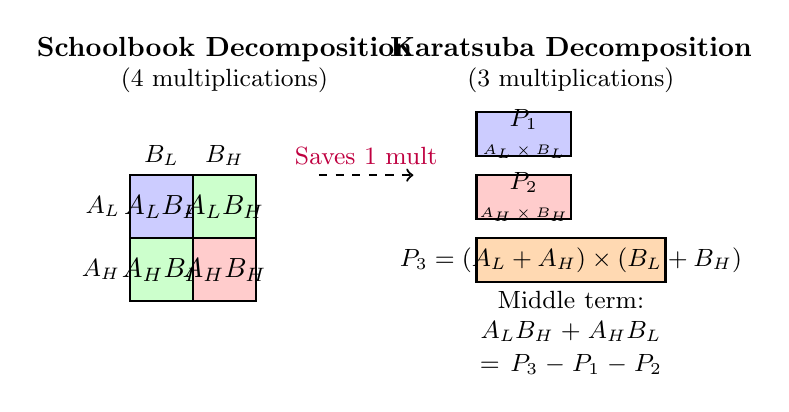
\begin{tikzpicture}[scale=0.8]
    % Schoolbook Decomposition (4 tiles)
    \node at (0, 3.5) {\textbf{Schoolbook Decomposition}};
    \node at (0, 3) {\small (4 multiplications)};
    
    % Draw 2x2 grid for schoolbook
    \draw[thick, fill=blue!20] (-1.5, 0.5) rectangle (-0.5, 1.5);
    \node at (-1, 1) {$A_L B_L$};
    
    \draw[thick, fill=green!20] (-0.5, 0.5) rectangle (0.5, 1.5);
    \node at (0, 1) {$A_L B_H$};
    
    \draw[thick, fill=green!20] (-1.5, -0.5) rectangle (-0.5, 0.5);
    \node at (-1, 0) {$A_H B_L$};
    
    \draw[thick, fill=red!20] (-0.5, -0.5) rectangle (0.5, 0.5);
    \node at (0, 0) {$A_H B_H$};
    
    % Labels
    \node[above] at (-1, 1.5) {\small $B_L$};
    \node[above] at (0, 1.5) {\small $B_H$};
    \node[left] at (-1.5, 1) {\small $A_L$};
    \node[left] at (-1.5, 0) {\small $A_H$};
    
    % Karatsuba Decomposition (3 tiles)
    \node at (5.5, 3.5) {\textbf{Karatsuba Decomposition}};
    \node at (5.5, 3) {\small (3 multiplications)};
    
    % Draw 3 separate tiles
    \draw[thick, fill=blue!20] (4, 1.8) rectangle (5.5, 2.5);
    \node[align=center] at (4.75, 2.15) {\small $P_1$\\[-2pt]\tiny $A_L \times B_L$};
    
    \draw[thick, fill=red!20] (4, 0.8) rectangle (5.5, 1.5);
    \node[align=center] at (4.75, 1.15) {\small $P_2$\\[-2pt]\tiny $A_H \times B_H$};
    
    \draw[thick, fill=orange!30] (4, -0.2) rectangle (7, 0.5);
    \node[align=center] at (5.5, 0.15) {\small $P_3 = (A_L + A_H) \times (B_L + B_H)$};
    
    % Middle term recovery
    \node[align=center, text width=3cm] at (5.5, -1) {\small Middle term:\\$A_L B_H + A_H B_L$\\$= P_3 - P_1 - P_2$};
    
    % Arrow showing saving
    \draw[->, thick, dashed] (1.5, 1.5) -- (3, 1.5) node[midway, above] {\small \textcolor{purple}{Saves 1 mult}};
\end{tikzpicture}
\caption{Comparison of Schoolbook and Karatsuba decomposition schemes. Schoolbook requires 4 multiplications for the four partial products, while Karatsuba cleverly reduces this to 3 multiplications by computing the middle term indirectly through $P_3 - P_1 - P_2$.}
\label{fig:decomposition_comparison}
\end{figure}
